
\newcommand{\csubfloat}[2][]{%
  \makebox[0pt]{\subfloat[#1]{#2}}%
}
\newcommand{\centerhfill}[1][\quad]{\hspace{\stretch{0.5}}#1\hspace{\stretch{0.5}}}

\begin{figure*}[bt]
\hspace{-1cm}
\begin{centering}
\makebox[\textwidth]{\makebox[1.25\textwidth]{
\begin{minipage}{0.3\textwidth}\centering
\subfloat[Compressed length against input length]{{
    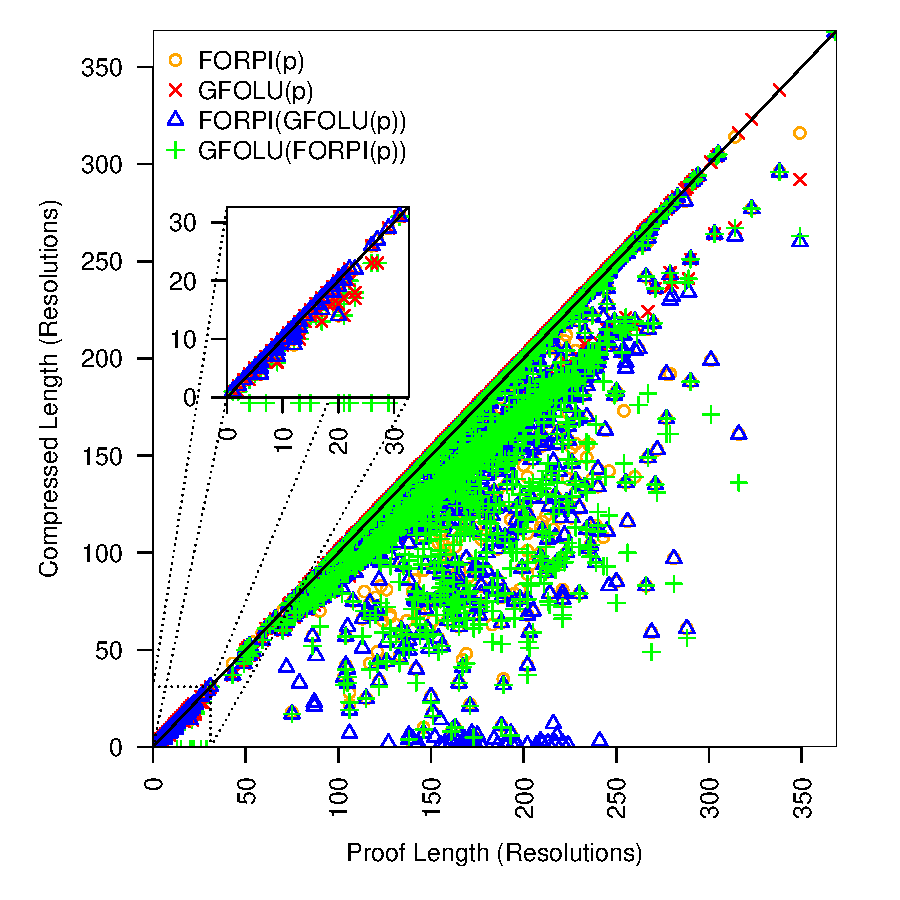
\includegraphics[scale=0.4]{images-new/combined-all-res-length-vs-compressed-res-length.pdf}%
    }}
 \end{minipage}\hfill
\begin{minipage}{0.3\textwidth}\centering
\subfloat[\FORPI(\GFOLU(p)) vs. \GFOLU(\FORPI(p))]{{
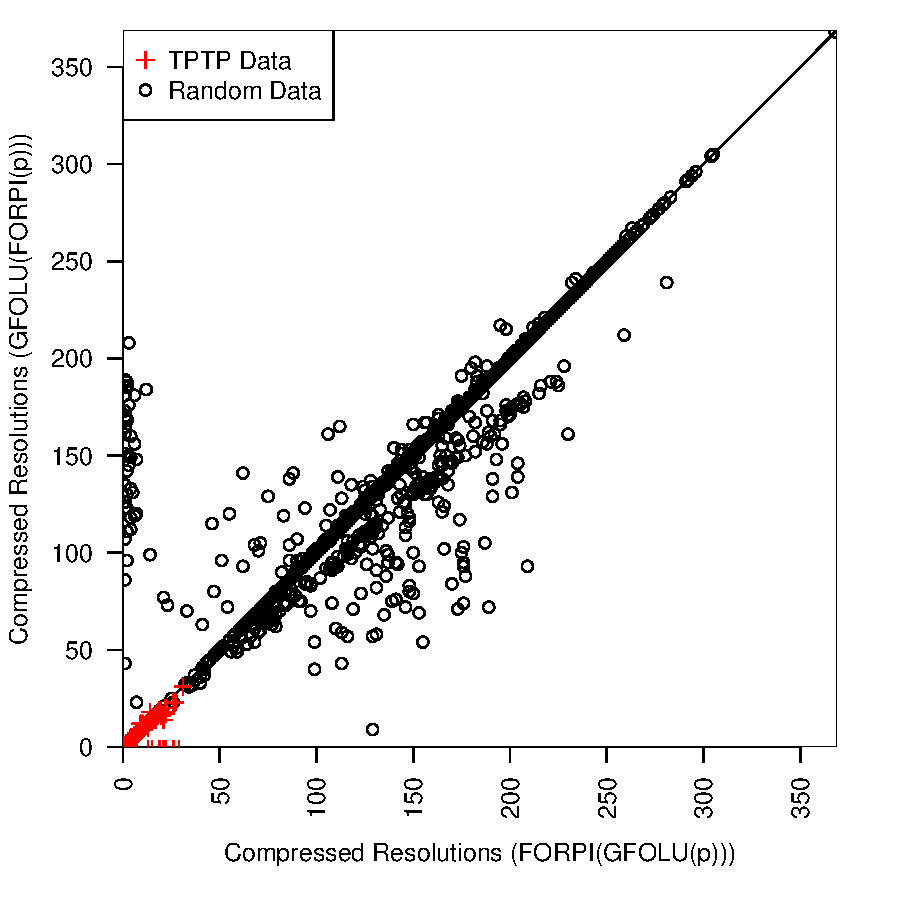
\includegraphics[scale=0.4]{images-new/combined-alg-res.pdf}%
}}
 \end{minipage}\hfill
\begin{minipage}{0.3\textwidth}\centering
\subfloat[Cumulative proof compression]{{
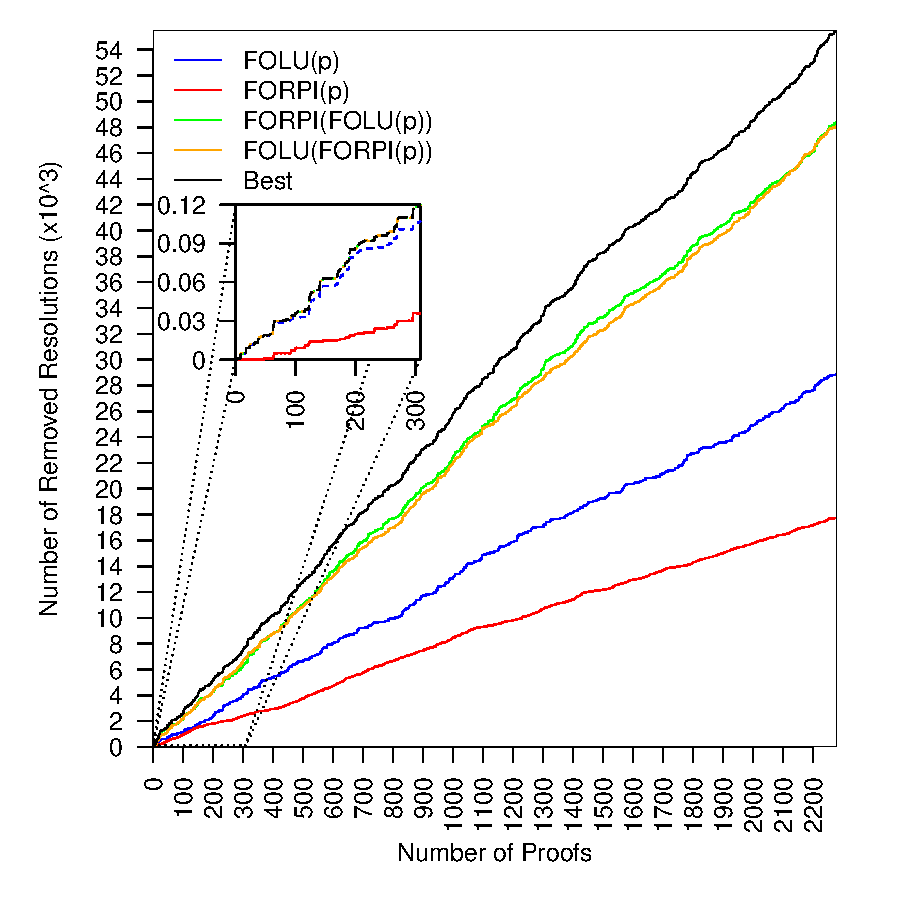
\includegraphics[scale=0.4]{images-new/combined-all-cumulative-res-nodes-diff.pdf}%
}}
 \end{minipage}
 }}\end{centering}
 \caption{\GFOLU \& \FORPI Combination Results}
\label{fig:ex}
\end{figure*}
